\documentclass{sigchi}


%% EXAMPLE BEGIN -- HOW TO OVERRIDE THE DEFAULT COPYRIGHT STRIP -- (July 22, 2013 - Paul Baumann)
% \toappear{Permission to make digital or hard copies of all or part of this work for personal or classroom use is      granted without fee provided that copies are not made or distributed for profit or commercial advantage and that copies bear this notice and the full citation on the first page. Copyrights for components of this work owned by others than ACM must be honored. Abstracting with credit is permitted. To copy otherwise, or republish, to post on servers or to redistribute to lists, requires prior specific permission and/or a fee. Request permissions from permissions@acm.org. \\
% {\emph{CHI'14}}, April 26--May 1, 2014, Toronto, Canada. \\
% Copyright \copyright~2014 ACM ISBN/14/04...\$15.00. \\
% DOI string from ACM form confirmation}
%% EXAMPLE END -- HOW TO OVERRIDE THE DEFAULT COPYRIGHT STRIP -- (July 22, 2013 - Paul Baumann)


% Arabic page numbers for submission.  Remove this line to eliminate
% page numbers for the camera ready copy 

%\pagenumbering{arabic}

% Load basic packages
\usepackage{balance}  % to better equalize the last page
\usepackage{graphics} % for EPS, load graphicx instead 
%\usepackage[T1]{fontenc}
\usepackage{txfonts}
\usepackage{times}    % comment if you want LaTeX's default font
\usepackage[pdftex]{hyperref}
% \usepackage{url}      % llt: nicely formatted URLs
\usepackage{color}
\usepackage{textcomp}
\usepackage{booktabs}
\usepackage{ccicons}
\usepackage{todonotes}

\usepackage{subcaption}


% llt: Define a global style for URLs, rather that the default one
\makeatletter
\def\url@leostyle{%
  \@ifundefined{selectfont}{\def\UrlFont{\sf}}{\def\UrlFont{\small\bf\ttfamily}}}
\makeatother
\urlstyle{leo}

% To make various LaTeX processors do the right thing with page size.
\def\pprw{8.5in}
\def\pprh{11in}
\special{papersize=\pprw,\pprh}
\setlength{\paperwidth}{\pprw}
\setlength{\paperheight}{\pprh}
\setlength{\pdfpagewidth}{\pprw}
\setlength{\pdfpageheight}{\pprh}

% Make sure hyperref comes last of your loaded packages, to give it a
% fighting chance of not being over-written, since its job is to
% redefine many LaTeX commands.
\definecolor{linkColor}{RGB}{6,125,233}
\hypersetup{%
  pdftitle={SIGCHI Conference Proceedings Format},
  pdfauthor={LaTeX},
  pdfkeywords={SIGCHI, proceedings, archival format},
  bookmarksnumbered,
  pdfstartview={FitH},
  colorlinks,
  citecolor=black,
  filecolor=black,
  linkcolor=black,
  urlcolor=linkColor,
  breaklinks=true,
}

% create a shortcut to typeset table headings
% \newcommand\tabhead[1]{\small\textbf{#1}}

% End of preamble. Here it comes the document.
  \begin{document}

%\title{Mining interaction log data in long-term practice-led research}
 
\title{Mining Interaction Log Data in a Creative Arts Practice using Transition Matrices}

\numberofauthors{3}
\author{%
  \alignauthor{1st Author Name\\
    \affaddr{Affiliation}\\
    \affaddr{City, Country}\\
    \email{e-mail address}}\\
  \alignauthor{3rd Author Name\\
    \affaddr{Affiliation}\\
    \affaddr{City, Country}\\
    \email{e-mail address}}\\
     \alignauthor{4th Author Name\\
    \affaddr{Affiliation}\\
    \affaddr{City, Country}\\
    \email{e-mail address}}\\
}

\maketitle

\begin{abstract}
  In this note we present an analysis of an interaction data archive
  associated with a long-term practice-led research program
  investigating ensemble musical performance practice on touch
  screens. We use transition matrix measures to distinguish between
  sessions of different contexts, and the internal structure of these
  sessions. The data analysis proceeds by first classifying these data
  into higher level gesture types and summarising the performers'
  transitions between these gestures. We find that two
  transition-matrix measures, flux, and entropy, can be used to
  distinguish different performance types and contexts, as well as the
  internal structure of the performances in our corpus.
\end{abstract}

\keywords{  
  Creativity Support Tools;
  Collaborative Interaction;
  Methodology}

\category{H.5.5.}{Information Interfaces and Presentation (e.g.
  HCI)}{Sound and Music Computing}[Methodologies and techniques]

\section{Introduction}

\begin{figure*}
  \centering
  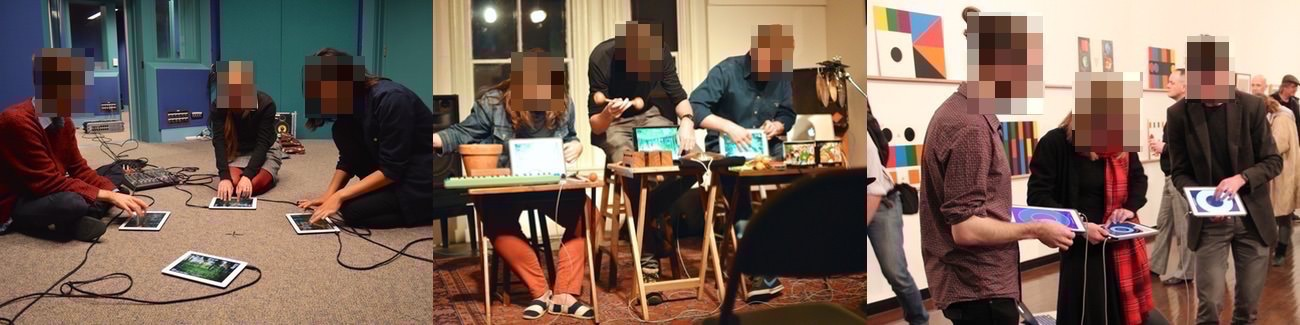
\includegraphics[width=\linewidth]{figures/three-performance-contexts}
  \caption{Collaborative musical interaction with our touch-screen
    interfaces in two different {\em contexts} and two different {\em
      instrumentations}: (left to right) a rehearsal with iPads only,
    concert performance with iPads and percussion instruments, and
    concert performance with iPads
    only.\label{fig:three-performance-contexts}}
\end{figure*}


Modern computing devices and interfaces continue to present
opportunities to support new kinds of creative expression and
collaborative interaction~\cite{Resnick:2005yu}. However, it has been
acknowledged that understanding and evaluating interfaces in creative
contexts can be very challenging~\cite{Shneiderman:2007qv}. This problem is
even more pronounced in artistic \emph{performance}, where subjective
interface evaluation through questionnaires or interviews may be both
practically difficult and culturally inappropriate. However, when an artistic interface
is digital, it becomes possible to log artistic performances and these
logs can be used for curation and
preservation~\cite{England:2014ys}. A question we address is: can this log data
be used to understand and support a
broader creative-practice-led research program?

In this note we will show how an archive of collaborative performance
logs can be subjected to a quantitative analysis based on
transition probabilities between gestural states. We will demonstrate
that two measures on transition matrices, flux and entropy, show
significant differences between different kinds of performances, and
give insight into the internal structure of these performances.

Our archive of interaction data-logs has been accumulated to support a
long-term, practice-led, research program into simple iPad interfaces
for group music-making. Over a period of more than two years (April
2013--June 2015), we collected data from group music-making sessions
where the participants used our custom-built, touch-screen apps on
Apple iPad devices. Although several different apps have been included
in our corpus, they shared a common mode of free-form touch
interaction where tapping produced short sounds and swirling or
swiping produced long sounds. Apart from these similarities, the apps
featured a variety of sound palettes, different kinds of visual
feedback, and different kinds of networked interactions (between the
iPads in an ensemble and with a central server).

In all of our 95 interaction sessions, every touch interaction---
touches begin, touches move, touches end ---was time-stamped and
logged to disk for later analysis. These sessions included {\em rehearsals} without an
audience, as well as {\em concerts}, in front of a live audience, where 
performative goals were paramount. They also included a number of {\em
  recording} sessions
for the purposes of formally-structured HCI experiments. In the recording
sessions, the performers were also interviewed and surveyed-- something which would have 
been disruptive and inappropriate for the concerts. Survey and interview data were not part of the
corpus. 
Some of the sessions were
iPad-only and others used iPads together with other acoustic
percussion instruments. Although the majority of the sessions were
free-form improvisations, a number of rehearsals and performances
involved composed pieces where the musicians read and performed
percussion notation using the apps.
Some of these session contexts are are shown
Figure~\ref{fig:three-performance-contexts} and other descriptive
statistics about the corpus are shown in Table \ref{corpus-table}.
In our corpus, the median length of sessions is 7m26s and the median
number of participants per ensemble is four. Each session record is
labelled with metadata about its \emph{context} (concert,
rehearsal, recording), its \emph{type} (improvisation or composition),
and its \emph{instrumentation} (iPads-only, or iPads with acoustic
percussion). The distribution of recorded sessions by context and type
is shown in Figure \ref{fig:count-data}.


% It is a feature of creative expression in the arts that highly skilled
% practitioners exploit simple tools to produce works of beauty whether
% it be static paintings or dynamic performance. 
% In previous work~\cite{Martin:2014cr} researchers have shown that
% trained percussionists can exploit a very simple iPad interface to
% discover new categories of musical gestures.
% In that paper, iPad apps
% were studied where tapping was mapped to produce produced short
% sounds, while swiping produced long sounds with the volume
% proportional to the velocity of the moving touch point. 
% It turned out that trained percussionists working together in an
% ensemble were able to discover and repeatedly make use of five macro
% gestures made up of taps and swipes: fast taps, slow taps, random
% taps, short swipes and swirls. This process of discovery of
% interesting musical gestures from a simple interface is analogous to
% what percussionists do with acoustic instruments -- drums and bowls
% and bells are often tapped, stroked and hit in novel ways to
% communicate meaning and emotion through music~\cite{Schick:2006fk}.

\begin{table}
\centering
\begin{tabular}{l|llll}
\hline
            & Total & Min  & Median   & Max     \\ 
\hline
N           & 95    &      &          &         \\
%Record size & 306MB     &         &        &   \\
Length & 13H9M19S & 1M19S & 7M26S & 22M20S \\
Participants& 353   & 2    & 4        & 9        \\
Flux &   & 0.02239 & 0.1445 & 0.3246\\
Entropy &   & 0.7683 & 3.342 & 4.442\\          
\hline
\end{tabular}
\caption{
  Representative statistics from the corpus of musical touch-screen
  interaction sessions described in this note.  Each record in the corpus
  consists of low level touch-data recorded in CSV format. 
  Many of the participants were
  present in multiple sessions, but this data was not tracked.\label{corpus-table}}
\end{table}

\section{Macro Gestures and Transition Matrices}

A useful way of modelling user interfaces is to consider their
theoretical configurations as state vectors and to deploy the methods
of matrix algebra to describe transitions between these states during
an interaction sequence~\cite{Thimbleby:2001kq, Thimbleby:2004fj}. An
inverted approach is to record users' interactions and manually code
interaction states to produce a transition model. This method has been
applied to usability analysis of many applications outside of the creative arts, for example~\cite{Kannampallil:2007fp}
studied resource-planning software for
security applications and used the transition
probability matrix of these state-sequences to draw
conclusions about the nature of interactions with that software. As an example from the creative
arts, protocols obtained from a computer interface for ``live coding''
computer music have been  coded as states and analysed using
transition matrices~\cite{Swift:2014tya} in both the textual (editing) and
musical dimensions, in order to arrive at conclusions regarding
artistic style.

In our corpus of iPad musical performances, logs of low-level touch-data record each performer's micro-gestures. 
Because it has been
established that musical performances on touch-screens can contain 
vocabularies of continuous macro gestures that unfold over
several seconds of touch interaction~\cite{Martin:2014cr}, and that
gestural performances can be divided into sequences of such states~\cite{Pressing:1988uo}, these logs
 can be used identify a sequence of such states for each performer.
If a performers' touch interactions can be classified as belonging
to one of $m$ distinct states, then, over the course of a session, each
participant $X$ generates a length $N$ sequence of these interaction
states $X_n$ ($n = 1, \ldots, N$) which can be thought of as Markov
process.
If there is an (automated) classification process for identifying each
participant's state sequence from their interaction data, then we can
estimate the $m \times m$ transition matrix (TM), $P$, which characterises
this process by setting each entry, $p_{ij}$, to be the number of times
state $j$ follows state $i$ in the sequence. The transition activity
of the whole ensemble can be calculated by averaging the TM for each
performer. The matrix can be normalised so that the sum of all
elements is equal to one.

To generate state sequences for our corpus we have used an automated
method to sample the data at regular intervals and to classify the logs of touch events
into the nine continuous touch-screen gestures identified by Martin et
al~\cite{Martin:2015jk}. A Random Forest~\cite{Breiman:2001kx}
classifier\footnote{The Random Forest classifier used was from
  Python's Scikit-learn package\cite{scikit-learn}.} was applied to
5-second windows of touch-data in our corpus to provide chains of
gesture-states for each participant in each session. These chains can
be used to create $9 \times 9$ transition matrices for individual
performers and the whole ensemble in each session.

\section{Quantitative Transition Matrix Measures}
\label{sec:underst-impr-group}

While the interaction sessions recorded in our corpus were performed
by many different participants with varying experience levels, in
different contexts and on different instrumental setups, the common
interface and method of recording the data allows all the sessions to
be transformed into gesture sequences, and transition matrices. While
these matrices can be used to visualise the structure of individual
performances, as has been done in ~\cite{Swift:2014tya}, we also wish to extract quantitative
measures from these TMs to compare the large number of sessions in our
corpus.
To do this we calculate two high-level quantities from each session:
``flux'' and ``entropy''. The flux of a sequence is defined as the
ratio of state transitions (e.g. $A \rightarrow B$ where $A \neq B$),
to self transitions (e.g. $A \rightarrow A $). The flux of a TM $P$ is
given by: $\mathrm{flux}(P) = 1 - \mathrm{tr}(P)$ where the trace
$\mathrm{tr}(P)$ is the sum of the diagonal entries of $P$.
Intuitively, flux is a measure of how frequently the participant/group
changes state. Flux returns a value in the interval $[0,1]$ and will
return 0 when participants never change state, and 1 when participants
never stay in the same state for two measurements in a row.

Another, evocative measure that can be defined on a TM is its
entropy, defined in the information-theoretic\cite{Shannon:1948rt}
sense: $H(P) = -\sum_{i,j}p_{ij}\log_2(p_{ij})$. This measure
is small when the matrix is sparse, and largest when each matrix
element is equal. It offers a different perspective on collaborative
interactions than the flux measure by capturing the breadth of the
gestural space explored by the participants throughout the course of
an interaction. Consider a degenerate case of a participant who
alternates between just two states for a whole performance: the flux in
this case will be maximal ($\mathrm{flux}(P) = 1$) since there are no
self-transitions, (only $A \rightarrow B$ or $ B \rightarrow A$) even
though the participant has only used a small subset of the state
space. The entropy of this interaction, on the other hand, will be
low. Entropy, therefore, is a measure of how broad the participant's
exploration of the state space is in a given interaction.

In the rest of this note we will use these matrix measures to answer
two questions. First, do the transition matrix measures allow us to
distinguish between different performance contexts, types and
instrumental setups? Secondly, do these measures allow us further
insight into the internal structure of performances?

\begin{figure}
  \centering
  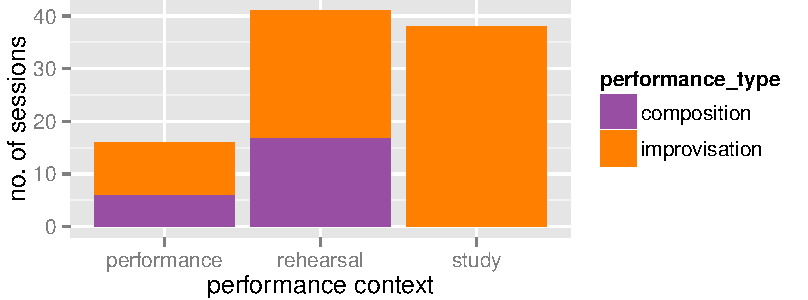
\includegraphics[width=\linewidth]{figures/sessions-count}
  \caption{Distribution of the sessions in our interaction corpus by
    session {\em context}. Improvisations or compositions were repeated
    several times in rehearsals and recording sessions but only performed
    once in concerts.
    \label{fig:count-data}}
\end{figure}


\subsection{Differentiating interaction sessions}
\label{differentiating-interaction-sessions}

\begin{figure} \centering
  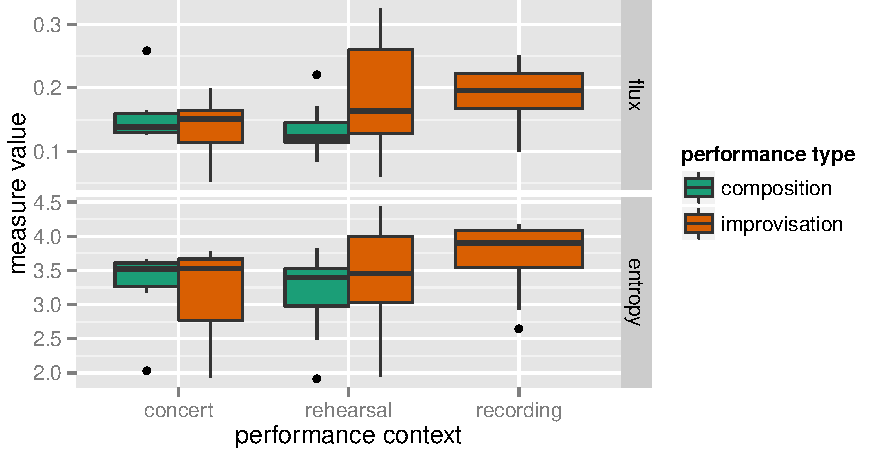
\includegraphics[width=\linewidth]{figures/context-flux-entropy-boxplot}
  \caption{Distributions of flux and entropy values by performance
context. Recording and rehearsal sessions had the highest flux for
improvisations. Compositions had lower
flux in rehearsals than concerts.
\label{fig:flux-entropy-boxplot}}
\end{figure}

The distribution of flux and entropy with respect to session {\em contexts} (concert,
rehearsal, recording),
{\em types} (improvisation or composition) and {\em instrumentation} (iPads-only, or iPads with acoustic
percussion) are shown in Figure
\ref{fig:flux-entropy-boxplot}. A three-way ANOVA procedure was
performed on the data set to find whether the metadata could
significantly predict the entropy and flux values.

All main effects on flux were found to be significant: session
context ($F(2,86) = 6.28, p < 0.01$), session type
($F(1,86) = 7.21, p < 0.01$), and instrumentation
($F(1,86) = 20.06, p < 0.001$). Significant interaction effects were
also found for session context and type
($F(1,86) = 6.18, p < 0.05$), and session context and
instrumentation ($F(1,86) = 10.48, p < 0.01$).

For entropy, significant main effects were found due to session
context ($F(2,86) = 12.10, p < 0.001$), and instrumentation
($F(1,86) = 25.86, p < 0.001$).
There was no main effect for session type although
 the interaction of session type and
instrumentation was found to be significant
($F(1,86) = 9.93, p<0.01$).

These tests show that the different interaction styles that might be
present in the various session contexts, types and instrumentations in our corpus
appear to be descriminated  by values of the flux and entropy of their transition
matrices.

% R> summary(aov(flux~performance_context*performance_type*instruments, perf.sessions))
%                                                  Df Sum Sq Mean Sq F value
% performance_context                               2 0.0267  0.0133    6.28
% performance_type                                  1 0.0153  0.0153    7.21
% instruments                                       1 0.0426  0.0426   20.06
% performance_context:performance_type              1 0.0131  0.0131    6.18
% performance_context:instruments                   1 0.0000  0.0000    0.02
% performance_type:instruments                      1 0.0223  0.0223   10.48
% performance_context:performance_type:instruments  1 0.0034  0.0034    1.62
% Residuals                                        86 0.1828  0.0021        
%                                                   Pr(>F)
% performance_context                               0.0028
% performance_type                                  0.0087
% instruments                                      2.3e-05
% performance_context:performance_type              0.0149
% performance_context:instruments                   0.8954
% performance_type:instruments                      0.0017
% performance_context:performance_type:instruments  0.2065
% Residuals                                               
% R> summary(aov(entropy~performance_context*performance_type*instruments, perf.sessions))
%                                                  Df Sum Sq Mean Sq F value
% performance_context                               2   5.10    2.55   12.10
% performance_type                                  1   0.31    0.31    1.48
% instruments                                       1   5.46    5.46   25.87
% performance_context:performance_type              1   0.21    0.21    0.99
% performance_context:instruments                   1   0.10    0.10    0.49
% performance_type:instruments                      1   2.09    2.09    9.93
% performance_context:performance_type:instruments  1   0.01    0.01    0.04
% Residuals                                        86  18.14    0.21        
%                                                   Pr(>F)
% performance_context                              2.3e-05
% performance_type                                  0.2267
% instruments                                      2.1e-06
% performance_context:performance_type              0.3224
% performance_context:instruments                   0.4878
% performance_type:instruments                      0.0022
% performance_context:performance_type:instruments  0.8396
% Residuals                                               
% R> 

\begin{figure*}[t!]
    \centering
    \begin{subfigure}[t]{0.5\linewidth}
        \centering
          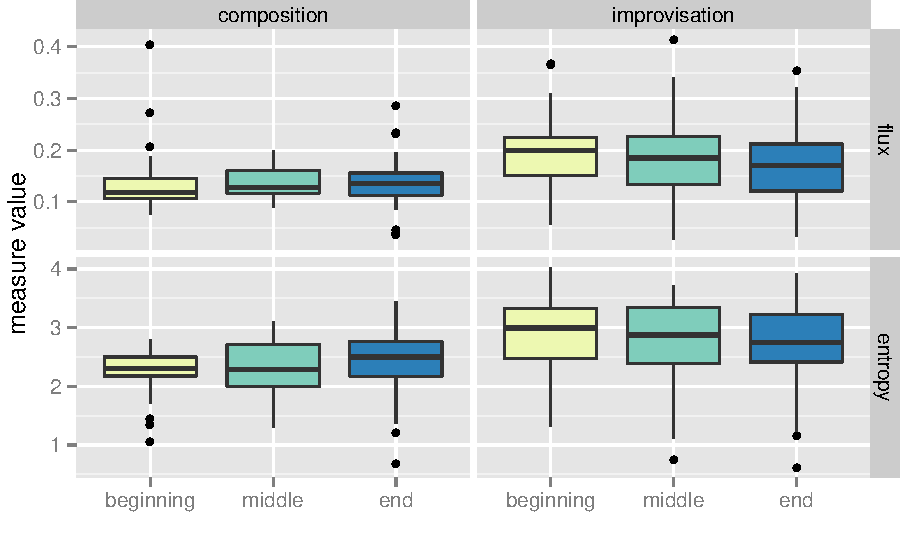
\includegraphics[width=\linewidth]{figures/type-section-flux-entropy}
          \caption{Sessions divided by performance type. \label{fig:type-section-flux-entropy}}
    \end{subfigure}%
    ~ 
    \begin{subfigure}[t]{0.5\linewidth}
        \centering
          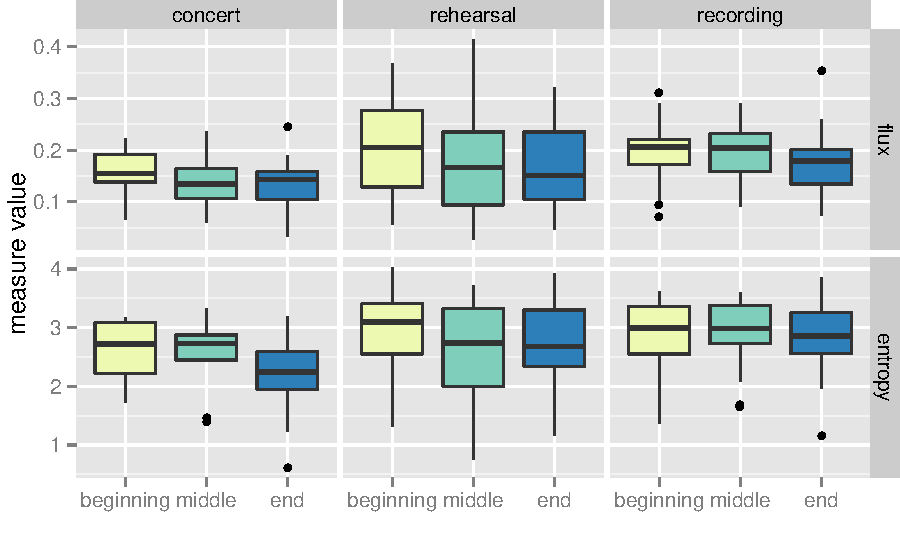
\includegraphics[width=\linewidth]{figures/context-section-flux-entropy}
          \caption{Improvisation performances divided by session context. \label{fig:context-section-flux-entropy}}
    \end{subfigure}
    \caption{The flux and entropy of different interaction sessions
      divided into beginning, middle, and end.}
\end{figure*}


\subsection{Breaking sessions into sections}

It appears from our data-mining results that both flux and entropy can be used to
differentiate between session styles and types, but can they be
used to understand some of the internal structure of sessions? Since Aristotle, a
classical model for understanding temporal art-forms is the three-phase
``beginning, middle, end'' structure~\cite{Aristotle:350rt}. To
investigate how this structure fits our corpus, we have divided the
gestural-sequences of each session into three equal sections and have calculated the
transition matrices given by each section.

Figure~\ref{fig:type-section-flux-entropy} shows that the flux and
entropy of compositions are much more stable across the three sections than  are
improvisations. This stability of compositions is to be
expected since performers use the same gestures in each rehearsal and
concert of written scores, however it may be that different
kinds of compositions could result in different structural
differences. Both measures have a downward trend through sections in
improvisations with Kruskal-Wallis tests showing a significant effect
of section on flux ($\chi^2(2)=5.8, p=0.05$). This could be explained
by performers entering an exploration stage at the start of an
improvisation, where they change gesture frequently to experiment with
different ideas. At the end of an improvisation, performers may change
gesture less frequently while ``winding up'' the concert performance.

The gestural change in improvisation can be further explored by
dividing the sessions by session context. Figure
\ref{fig:context-section-flux-entropy} shows this division for
improvisations only. In rehearsals and studies the distribution of
flux and entropy over sections has a similar shape, both measures drop
in the ending section of studies and after the beginning section in
rehearsals. In concerts however, flux drops after the beginning
while entropy drops substantially in the ending section. This
indicates a more constrained performance style in this closing
section, where performers transition between fewer gestures in the
final section of concert performances.

\subsection{Performance styles over time}

While the interaction sessions in our corpus have many different
contexts, they are all part of a program of artistic and HCI research
that has evolved over time. Figure \ref{fig:flux-entropy-through-time}
shows the values of flux and entropy for each session in the corpus.
Over the course of this data collection, different ensembles and
activities have been emphasised and some of these differences can be
seen as clusters of performances having similar fluxes and entropies in the
two plots. For instance, the earliest series of rehearsals and
concerts, from early 2013 until July 2014, 
had fluxes that were bounded between approximately 0.05 and 0.17.
Just before and after July 2014, fluxes were bounded between 0.1 and 0.26. Finally,
between early and mid 2015, fluxes were bounded between 0.08 and 0.32. Within these 
blocks of performances, distinct clusters can be identified. Clusters in the entropy plots
sometimes show similar trends to the fluxes and sometimes different. The higher
upper bounds of fluxes close to July 2015 relative to those a year earlier may indicate
the development of a more ``fluctuating'' style of performance. In the same period, the bound
of entropies remained more similar indicating that the total space of available gestures continued
to be explored in a relatively stable way. 

\begin{figure}
  \centering
  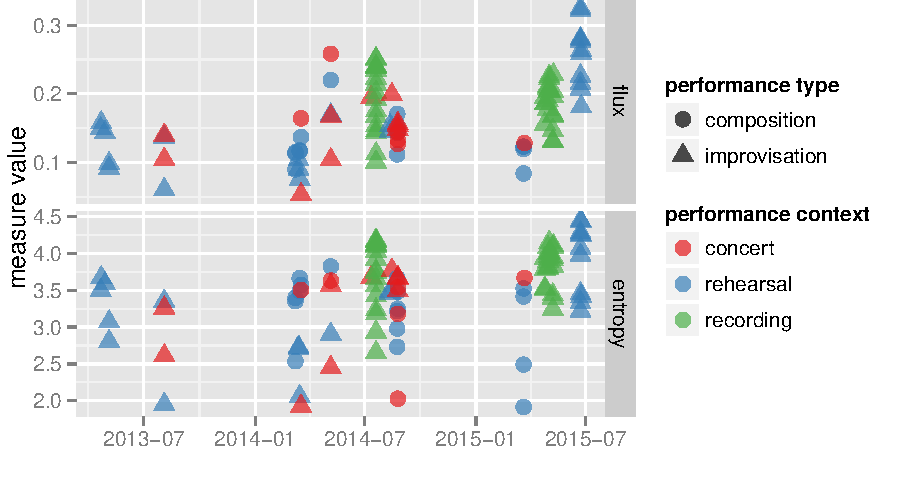
\includegraphics[width=\linewidth]{figures/flux-entropy-through-time}
  \caption{Distribution of flux and entropy values of sessions through time.
    Different performance styles are visible as clusters of similar
    flux regardless of session context.
    \label{fig:flux-entropy-through-time}}
\end{figure}

\section{Conclusions}

In this note we have applied transition matrices
to a data corpus of 95 collaborative musical performances using touch screens.
We have applied two simple matrix
measures, flux and entropy, to the data and have shown that
 both of these measures appear to 
have discriminatory power. Not only do these measures
differentiate between different types of sessions, and the internal
structure of these sessions, but they provide qualitative insight into the
performances. For improvised performances, it turns out that our results showed that concerts
had the lowest values of both flux and entropy, while recording sessions had
the highest. This may be due to the increased pressure on performers to take fewer risks
when improvising in front of an audience at a concert and indicates that perhaps rehearsals should 
emphasise the development of such risk-taking. 
Our results for the three phases of performance (beginning, middle, end)
revealed more variation in
improvisations than compositions. As a creative
 response to this finding, 
new works might be
composed that specifically explore and emphasise different gestural sequences across the three phases.

Our data-mining of interaction-logs from creative interfaces suggests
further approaches for future work.
Our flux and entropy measures have proven useful
in the analysis of our data corpus, but many other transition matrix
metrics might be found to be useful for these and different interaction data.
Our assumption of equal intervals for the beginning, middle and end of performances could be 
optimised with a goal to identifying a common, or even optimal, apportionment of time to each phase.  
A wide dissemination of corpuses such as ours could better support the replication of findings in HCI
research~\cite{Wilson:2011ve}. The macro-gestures that these
processes reveal could be used as the basis for ``transcoding'' new works of new media
art~\cite{Manovich:2002ly} from these data corpuses. 

%HCI researchers are increasingly concerned with interactions that
%happen in-the-wild, where the creative collaborations of many users
%may be recorded, but where conducting surveys or interviews is
%innapropriate. We suggest that analysing interaction-state transitions
%using matrices and simple measures can lead to new insights into HCI
%interactions outside the lab.


%\pagebreak
\bibliographystyle{SIGCHI-Reference-Format}
\bibliography{references}

\end{document}

%%% Local Variables:
%%% mode: latex
%%% TeX-master: t
%%% End:
